Have you ever wondered what goes on between the `A' you hit on your
keyboard, the `A' stored in your file, and the `A' that comes out of
your printer? Why that letter still comes out of the printer if the
file is printed by your friend in Greece who doesn't use the
letter~`A'? Maybe you know that `A' is character 41 in ascii; if you
put it on a web page, and it's watched by someone in Japan, why don't
they get character~41 in the Kanji alphabet? Do you remember the DOS
days when your Mac owning colleague would send you a file and what
were supposed to be accented characters would turn into smiley faces?
Have you ever pasted text from MS-Word into Emacs, and Emacs wanted to
save the document as UTF-8? Just what is that about?

All this, and more, will be explained in this article.

\Level 0 {History in one byte}

%\Level 1 {One-byte character sets; Ascii}

Somewhere in the depths of prehistory, people in the western world got
to agree on a standard for character codes
\index{ascii!7-bit}under~127, \index{ascii}\ascii, the American
Standard Code for Information Interchange.  This standard declares
that the letter~`A' is character number~41, so if your file contains
the bit pattern for~41 (which is~\texttt{00101001}), it will produce an
`A' when sent to the printer.

\ascii\ has a few nice properties, some of which were not shared by
another encoding scheme,
\index{ebcdic}\ebcdic\ (which was used almost exclusively by IBM):
\begin{itemize}
\item All letters are consecutive, making a test `is this a letter'
  easy to perform.
\item Uppercase and lowercase letters are at a distance of 32; this
  means that the Shift key on your keyboard simply toggles the sixth bit in
  the pattern of whatever key you are holding down.
\item The first 31 codes, everything below the space character, as
  well as position~127, are
  `\index{ascii!unprintable}unprintable', and can be used for such
  purposes as terminal cursor control.
\end{itemize}

The \index{ISO!646, 7-bit ascii}ISO 646 standard codified 7-bit \ascii,
but it left certain character positions (or `\index{code point}code
points') open for national variation. For instance, British usage put
a pound sign (\pounds) in the position of the dollar. The
\ascii\ character set was originally accepted as ANSI X3.4 in 1968.

%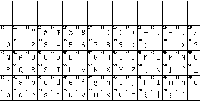
\includegraphics[scale=2.2]{ascii}
\begin{table}[p]
  \input ascii
  \caption{The \ascii\ table}
  \label{tab:ascii}
\end{table}
%\Level 1 {Code pages}

Since a computer organizes its bits in 8-bit bytes, and \ascii\ only
codified the codes under~128, this left the codes with the
\index{ascii!8-bit}high bit set (`\index{ascii!extended}extended
\ascii') undefined, and different manufacturers of computer equipment
came up with their own way of filling them in. These standards were
called `\index{code page}code pages', and IBM gave a standard
numbering to them. For instance, code page~437 is the MS-DOS code page
with accented characters for most European languages, 862~is DOS in
Israel, 737~is DOS for Greeks.

Here is cp473:\\
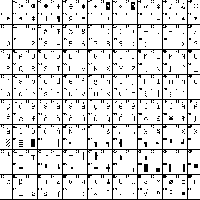
\includegraphics[scale=2.2]{dos437}

MacRoman:\\
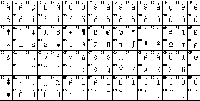
\includegraphics[scale=2.2]{macroman}

and Microsoft cp1252:\\
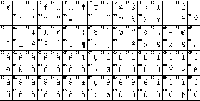
\includegraphics[scale=2.2]{winlatin1}

(Find more code pages are displayed on~\cite{codepage}.)
\begin{comment}
These diagrams can be generated from Unicode mapping tables, which
look like
\begin{verbatim}
=20     U+0020  SPACE
=21     U+0021  EXCLAMATION MARK
=22     U+0022  QUOTATION MARK
...
=A3     U+00A3  POUND SIGN
=A4     U+20AC  EURO SIGN
=A5     U+00A5  YEN SIGN
...
\end{verbatim}
\end{comment}

The international variants were standardized as ISO 646-DE (German),
646-DK (Danish), et cetera. Originally, the dollar sign could still be
replaced by the currency symbol, but after a 1991 revision the dollar
is now the only possibility.

%\Level 1 {The ISO 8859 standard}

The
different code pages were ultimately standardized as \index{ISO!8859,
Latin alphabets}ISO~8859, with such popular code pages as
8859-\nobreak1 (`Latin~1') for western European,

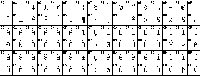
\includegraphics[scale=2.2]{latin1}

8859-\nobreak2 for
eastern European, and 8859-\nobreak5 for Cyrillic.

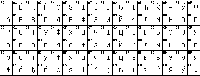
\includegraphics[scale=2.2]{8859-cyrillic}

These ISO standards
explicitly left the first 32 extended positions undefined. 
% Microsoft
% code page~1252 uses ISO 8859-\nobreak1.

Reading material: The history of \ascii\ out of
telegraph codes~\cite{history-of-ascii}. A~history, paying
attention to multilingual use~\cite{character-codes-europe-asia}.
Bob Bemer, the `father of ascii'~\cite{bobbemer}.
A~detailed discussion of ISO 8859, Latin-1~\cite{latin1}.

\Level 0 {Character sets and encodings}

As you can tell from the introduction, there is quite a bit of
confusion possible between characters and representations or
encodings. Let us clear up the concepts a little.

Informally, the term `character set' (also `character code' or `code')
used to mean something like `a~table of
bytes, each with a character shape'. With only the English alphabet to
deal with that is a good enough definition. These days, much more general
cases are handled, mapping one octet into several characters, or
several octets into one character. The definition has changed
accordingly:
\begin{quote}
A \index{charset}\emph{charset} is
a method of   converting a sequence of octets into a sequence of
characters.  This   conversion may also optionally produce additional
control information   such as directionality indicators.
\end{quote}
(From RFC 2978) A~conversion the other way may not exist, since
different octet combinations may map to the same character.  Another
complicating factor is the possibility of switching between character
sets; for instance, \index{ISO 2022}ISO 2022-JP is the standard
\ascii\ character set, but the escape sequence \verb+ESC $ @+ switches
to JIS X 0208-1978.

To disentangle the concepts behind encoding, we need to introduce a
couple of levels:
\begin{description}
\item[ACR] Abstract Character Repertoire: the set of characters to be
  encoded; for example, some alphabet or symbol set. This is an
  unordered set of characters, which can be fixed (the contents of ISO
  8859-1), or open (the contents of Unicode).
\item[CCS] Coded Character Set: a mapping from an abstract character
  repertoire to a set of nonnegative integers. This is what is meant
  by `encoding', `character set definition', or `code page'; the
  integer assigned to a character is its `\index{code point}code
  point'.

  There used to be a drive towards unambiguous abstract character
  names across repertoires and encodings, but Unicode ended this, as
  it provides (or aims to provide) more or less a complete list of
  every character on earth.
\item[CEF] Character Encoding Form: a mapping from a set of
  nonnegative integers that are elements of a CCS to a set of
  sequences of particular code units. A~`\index{code unit}code unit'
  is an integer of a specific binary width, for instance 8 or~16
  bits. A~CEF then maps the code points of a coded character set into
  sequences of code point, and these sequences can be of different
  lengths inside one code page. For instance 
 \ascii\ uses a single 7-bit unit; 
  UTF-8 uses one to four 8-bit units.
  We will discuss the UTF encodings below.
\item[CES] Character Encoding Scheme: a reversible transformation from
  a set of sequences of code units (from one or more CEFs to a
  serialized sequence of bytes. In single-byte cases such as \ascii\
  and UTF-8 this mapping is trivial. With the two-byte scheme UCS-2
  there is a single `\index{byte order mark}byte order mark', after
  which the code units are trivially mapped to bytes. On the other
  hand, ISO~2022, which uses escape sequences to switch between
  different encodings, is a complicated CES.
\end{description}
Additionally, there are the concepts of
\begin{description}
\item[CM] Character Map: a mapping from sequences of members of an
  abstract character repertoire to serialized sequences of bytes
  bridging all four levels in a single operation. These maps are what
  gets assigned MIBenum values by IANA; see section~\ref{sec:mibenum}.
\item[TES] Transfer Encoding Syntax: a reversible transform of encoded
  data. This data may or may not contain textual data. Examples of a
  TES are base64, uuencode, and quoted-printable, which all transform
  a byte stream to avoid certain values.
\end{description}

\Level 0 {Unicode and UTF encodings}
\label{sec:unicode}

The systems above functioned quite well as long as you stuck to one
language or writing system. Poor dictionary makers. More or less
simultaneously two efforts started that aimed to incorporate all the
world's character sets in one standard: Unicode standard (originally 2-byte),
and \index{ISO!10646, Unicode}ISO~10646 (oringally 4-byte). Unicode was
extended further, so that it has all code points up to~\n{10FFFFF}, which is
slightly over a million. 


\index{ISO!10646, Unicode}Two international standards organizations,
the Unicode Consortium and ISO/IEC JTC1/SC2,
started designing a universal standard that was to be a
superset of all existing character sets. These standards are now
synchronized. Unicode has elements
that are not in 10646, but they are compatible where it concerns
straight character encoding.

ISO 10646 defines UCS, the `\index{UCS, Universal Character
  Set}Universal Character Set'. This is in essence a table of official
names
and code numbers for characters. Unicode adds to this rules for hyphenation,
bi-directional writing, and more.

The full Unicode list of code points can be found online, broken down by
blocks~\cite{unicode-fileformat}, and 
downloadable~\cite{unicode-download}.

\Level 1 {BMP and earlier Unicode subplanes}

Characters in Unicode are mostly denoted hexadecimally as~\n{U+wxyz},
for instance \n{U+0041} is `Latin Capital Letter~A'.
The range \n{U+0000}--\n{U+007F} (0--127) is identical to US-ASCII
(ISO 646 IRV), and \n{U+0000}--\n{U+00FF} (0--255) is identical to
Latin~1 (ISO 8859-1).

The original 2-byte subset is
now called `\index{BMP}BMP' for Basic Multilingual Plane, or
plane~0. These are the Unicode code points that are nonzero in the
last two bytes. Other `planes' have been defined that have one or more
bits set outside the last two bytes.

\begin{description}
\item[BMP] (Basic Multilingual Plane) The first plane defined in
  Unicode/ISO 10646, designed to include all scripts in active modern
  use. The BMP currently includes the Latin, Greek, Cyrillic,
  Devangari, hiragana, katakana, and Cherokee scripts, among others,
  and a large body of mathematical, APL-related, and other
  miscellaneous characters. Most of the Han ideographs in current use
  are present in the BMP, but due to the large number of ideographs,
  many were placed in the Supplementary Ideographic Plane.
\item[SMP] (Supplementary Multilingual Plane; plane~1) This contains
  mostly ancient writing systems. Some of these you'll have heard of,
  such as Linear~B, cuneiform, Aztec, and Maya; others are fairly
  obscure, such as Tangut, a language used in Central China between
  1000 and~1500.
\item[SIP] (Supplementary Ideographic Plane) The third plane (plane 2)
  defined in Unicode/ISO 10646, designed to hold all the ideographs
  descended from Chinese writing (mainly found in Vietnamese, Korean,
  Japanese and Chinese) that aren't found in the Basic Multilingual
  Plane. The BMP was supposed to hold all ideographs in modern use;
  unfortunately, many Chinese dialects (like Cantonese and Hong Kong
  Chinese) were overlooked; to write these, characters from the SIP
  are necessary. This is one reason even non-academic software must
  support characters outside the BMP.
\end{description}

\Level 1 {Unicode encodings}
\label{sec:uni-encoding}

Unicode is basically a numbered list of characters. When they are used
in a file, their numbers can be encoded in a number of ways. To name
the obvious example: if only the first 128 positions are used, the
long Unicode code point can be truncated to just one byte. Here are a
few encodings:
\begin{description}
\item[UTF-32] Little used: this is a four-byte encoding. (UTF stands
  for `UCS Transformation Format'.)
\item[UTF-16] A two-byte encoding. Its precursor, UCS-2, encoded the
  BMP; UTF-16 has a way of going beyond that to encode planes 1--16
  by using `surrogate pairs' of two-byte units.
\item[UTF-8] A one-byte scheme; details below.
\item[UTF-7] Another one-byte scheme, but now the high bit is always
  off. Certain byte values act as `escape', so that higher values can
  be encoded. Like UTF-1 and SCSU, this encoding is only of historical
  interest.
\end{description}

There is an important practical reason for a one-byte encoding such as
UTF-8. Multi-byte encodings such as
UCS-2 are wasteful of space, if only traditional \ascii\ is
needed. Furthermore, they would break software that is expecting to
walk through a file with~\verb-s++- and such. Also, they would
introduce many zero bytes in a file, which would play havoc with Unix
software that uses null-termination for strings. 

Then there would be
the problem of whether two bytes are stored in low-endian or
high-endian order. For this reason it was suggested to store \n{FE FF}
or \n{FF FE} at the beginning of each file as the `Unicode Byte Order
Mark'. Formally, \n{FEFF} is the Unicode `zero width nobreak space'
character, which can innocently be inserted anywhere. Conversely
\n{FFEF} is defined to be illegal, so encountering this is a sign that
bytes should be interpreted little-endian.
Of course this plays havoc with files such as shell scripts
which expect to find \verb+#!+ at the beginning of the file.

\Level 1 {UTF-8}

UTF-8, standardized as RFC~3629, is an encoding where the positions up
to 127 are encoded `as such'; higher numbers are encoded in groups of
2 to~6 bytes. (Tim Bray describes this as `kind of
racist'~\cite{bray-bytes}: the further east a language comes from, the
more overhead is involved in its encoding.)  In a multi-byte group,
the first byte is in the range 0xC0--0xFD (192--252). The next up to~5
bytes are in the range 0x80--0xBF (128--191, bit pattern starting
with~\n{10}). Note that $\n{8}=\n{1000}$ and $\n{B}=\n{1011}$, so the
highest two bits are always~\n{10}, leaving six bits for encoding).

\begin{quote}\begin{footnotesize}
\begin{ttfamily}\begin{tabular}{|l|llll|}
\hline
U-00000000 - U-0000007F&\textrm{7 bits}&
0xxxxxxx&&\\
U-00000080 - U-000007FF&$11=5+6$&
110xxxxx&10xxxxxx&\\
U-00000800 - U-0000FFFF&$16=4+2\times6$&
1110xxxx&10xxxxxx&10xxxxxx\\
U-00010000 - U-001FFFFF&$21=3+3\times6$&
11110xxx&\multicolumn{2}{l|}{10xxxxxx (3 times)}\\
U-00200000 - U-03FFFFFF&$26=2+4\times6$&
111110xx&\multicolumn{2}{l|}{10xxxxxx (4 times)}\\
U-04000000 - U-7FFFFFFF&$31=1+5\times6$&
1111110x&\multicolumn{2}{l|}{10xxxxxx (5 times)}\\\hline
  \end{tabular}
\end{ttfamily}
  \end{footnotesize}
\end{quote}

All bites in a multi-byte sequence have their high bit set.

\begin{594exercise}
Show that a UTF-8 parser will not miss more than two characters
if a byte becomes damaged (any number of bits arbitrarily changed).
\end{594exercise}

IETF documents such as
RFC~2277 require support for this encoding in internet
software. Readable introductions can be found all over the
internet~\cite{utf-faq}; see also the history of UTF-8~\cite{utf-history}.

\Level 1 {Unicode tidbits}

\Level 2 {Line breaking}

The Unicode standard describes line breaking: it has a mechanism for 
specifying tables of character pairs between which line breaks are
allowed or forbidden~\cite{unicode-tr14,unicode-line-breaking}.

\Level 2 {Bi-directional writing}

Most scripts are left-to-right, but Arabic and Hebrew run
right-to-left. Characters in a file are stored in `logical order', and
usually it is clear in which direction to render them, even if they
are used mixed. Letters have a `strong' directionality: unless
overridden, they will be displayed in their natural direction. The
first letter of a paragraph with strong direction determines the main
direction of that paragraph~\cite{unicode-tr9}.

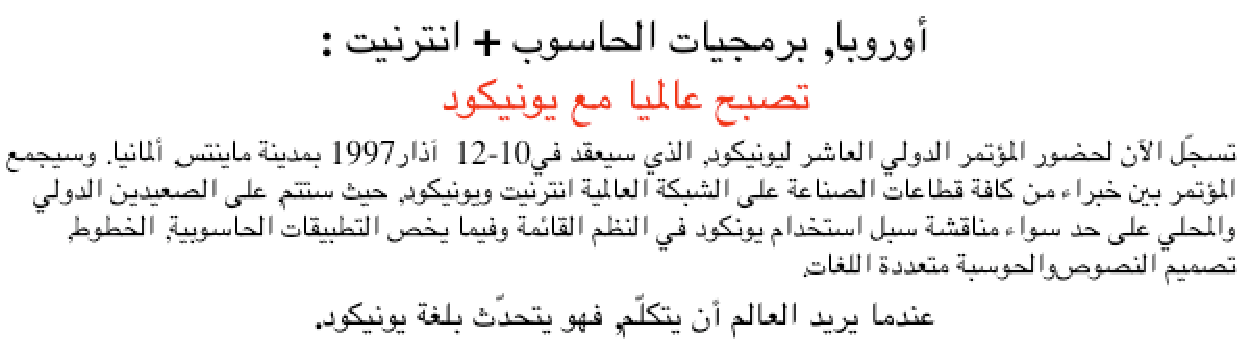
\includegraphics[scale=.6]{arabic-date}

However, when differently directional texts are
embedded, some explicit help is needed. The problem arises with
letters that have only weak directionality. The following is a sketch
of a problematic case.
\begin{quote}
Memory:  he said "I NEED WATER!", and expired.\\
Display: he said "RETAW DEEN I!", and expired.
\end{quote}
If the exclamation mark is to be part of the Arabic quotation, then
the user can select the text `I NEED WATER!' and explicitly mark it as
embedded Arabic (\n{<RLE>} is Right-Left Embedding; \n{<PDF>} Pop
Directional Format), which produces the following result:
\begin{quote}
Memory:  he said "\n{<RLE>}I NEED WATER!\n{<PDF>}", and expired.\\
Display: he said "!RETAW DEEN I", and expired.
\end{quote}
A simpler method of doing this is to place a Right Directional Mark
\n{<RLM>} after the exclamation mark. Since the exclamation mark is now
not on a directional boundary, this produces the correct result.
\begin{quote}
Memory:  he said "I NEED WATER!\n{<RLM>}", and expired.\\
Display: he said "!RETAW DEEN I", and expired.
\end{quote}


\Level 1 {Unicode and oriental languages}
\label{sec:unihan}

`Han unification' is the Unicode strategy of saving space in the
oriental languages (traditional Chinese, simplified Chinese, Japanese,
Korean: `CJK') by recognizing common characters. This idea is not
uncontroversial~\cite{han-unification}.

\Level 0 {Further tidbits}

\Level 1 {A bootstrapping problem}
\label{sec:mibenum}

In order to know how to interpret a file, you need to know what
character set it uses. This problem also occurs in MIME mail encoding
(section~\ref{sec:mime}), which can use many character sets.  Names
and numbers for character sets are standardized by \index{IANA}IANA:
the Internet Assigned Names Authority~\cite{iana}. However, in what
character set do you write this name down?

Fortunately, everyone agrees on (7-bit) \ascii, so that is what is
used. A~name can be up to 40 characters from us-ascii.

As an example, here is the iana definition of \ascii:
\begin{itemize}
\item[name] \n{ANSI_X3.4-1968}
\item[reference] RFC1345,KXS2
\item[MIBenum] 3
\item[source] ECMA registry
\item[aliases] \n{iso-ir-6}, \n{ANSI_X3.4-1986}, \n{ISO_646.irv:1991},
  \n{ASCII}, \n{ISO646-US}, \n{US-ASCII (preferred MIME name)},
  \n{us}, \n{IBM367}, \n{cp367}, \n{csASCII}
\end{itemize}
The \n{MIBenum} (Management Information Base) is a number assigned by
IANA\footnote{Apparently these numbers derive from the Printer MIB, RFC~1759.}.
The full list of character sets can be found oneline~\cite{iana-list},
and RFC 3808 is a memo that describes the IANA Charset MIB.

\Level 1 {Unicode in programming languages}

Before Unicode, a~system
called the `\index{DBCS}Double Byte Character Set' was invented 
to accomodate Asian languages, where
some characters were stored in one, others in two bytes. This is very
messy, since you can not simply write \verb-s++- or \verb+s--+ to
traverse a string. Instead you have to use functions from some library
that understands these encodings. While this system is now only of
historical interest, the string handling problem is back in force with
UTF-8.

Many modern languages (Python, C99) have support for Unicode. In C99
(which is the new standard for~C) this is done through so-called `wide
characters'. For instance, \verb+L'x'+ is a wide character and
\verb+L"xyz"+ is a string of side characters. Such strings can be
manipulated through equivalents of the normal string library. For
instance, \verb+wcscpy+ acts like \verb+strcpy+ but on wide strings.
General Unicode characters can be represented as \verb+\u0000+ for
4-byte and \verb+\U00000000+ for up to 8-byte characters.

The two-byte UTF-16 encoding is popular among programmers, since it
can handle almost any practically encountered character without
extensions to longer byte sequences.

\Level 1 {Character codes in HTML}

HTML can access unusual characters in several ways:
\begin{itemize}
\item With a decimal numerical code: \verb+&#32;+ is a space
  token. (HTML~4 supports hexadecimal codes.)
\item With a vaguely symbolic name~\cite{html-names,html-chars}:
  \verb+&copy;+ is the copyright symbol.
\item The more interesting way is to use an encoding such as UTF-8
  (section~\ref{sec:uni-encoding}) for the file. For this it would be
  nice if the server could state that the file is
\begin{verbatim}
Content-type: text/html;charset=utf-8
\end{verbatim}
  but it is also all right if the file starts with
\begin{verbatim}
<META HTTP-EQUIV="Content-Type" CONTENT="text/html;charset=utf-8">
\end{verbatim}
\end{itemize}

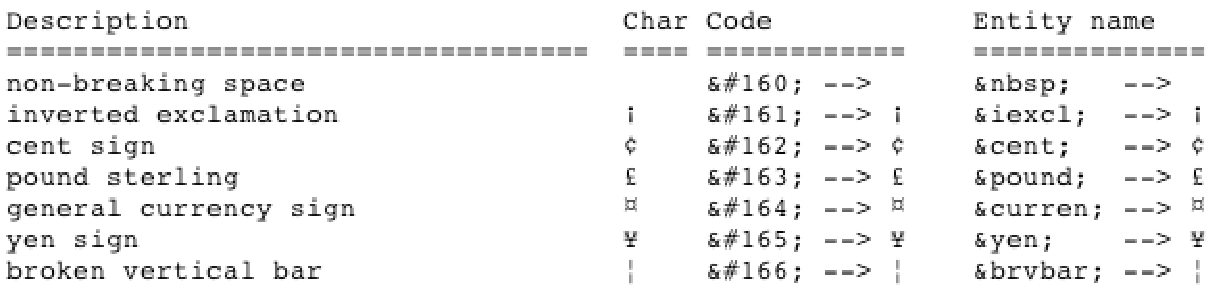
\includegraphics[scale=.6]{latin1-html}

It is requirement that user agents can at least parse the \n{charset}
parameter, which means they have to understand us-ascii.

Open this link in your browser, and additionally view the source:
\url{http://www.unicode.org/unicode/iuc10/x-utf8.html}. How well does
your software deal with it?

%See also section~\ref{sec:unicode-font}.

\Level 1 {Keyboards and control characters}

Unprintable ascii codes are accessible through the control modifier
key; for this reason they are also called `\index{ascii!control
  codes}control codes' or control characters. The control key,
combined with a regular key, zeros bits 2 and~3 of the ascii code of
that key. For instance, you can hit \n{Ctrl-[} to get
\n{Esc}.

The way key presses generate characters is typically controlled in
software. This mapping from keyboard \index{scan code}scan codes to
7~or~8-bit characters is called a `keyboard', and can be changed
dynamically in most operating systems.

Using the modifier keys, one can generate more keystrokes than can be
described in 8 bits, so keyboards can send an \index{escape
  sequence}`escape sequence': one escape character followed by one or
more regular characters. The escape character is mostly ascii NULL or
ESC~\cite{scancodes}.

\Level 1 {Characters in email}\label{sec:mime}

The protocols for internet mail are based on `7-bit \ascii', that is,
the high bit in every byte transmitted is supposed to be off. This is
a problem for any message that has text outside of \ascii, such as
when accented characters from the various ISO 8859 character sets are
used. It also makes transmitting binary data such as images
impossible. For this reason the `Multipurpose Internet Mail
Extensions' (MIME) were designed. MIME uses several encoding schemes,
such as base64 or printed quotable, to turn arbitrary data into 7-bit
ascii.

The email standard RFC 822 states that anything outside 7-bit ascii
has to be encoded with \n{uuencode}. This means that the sender and
recipient need decoding program; it is decidedly overkill if a message
is plain \ascii\ apart from a few accented characters.

The MIME protocol (RFC 2045 and 2046) inserts headers in a mail
message, stating for each message section the content type and the
encoding that is used for that section of the
message. These encodings are also used for attachments, in which case
the content type should give an indication what application can handle
the attachment after its decoding. `Helpful' mail programs that
automatically invoke such applications have been a source of Trojans
(malicious softwares) in the past.

\Level 1 {FTP}

FTP is a very old ARPA protocol for transferring files from one
computer to another. It knows `binary' and `text' mode: in binary mode
bytes are transferred without further interpretation, but the text
mode is concerned with files that contain lines of text.
Unfortunately, line ends are different between operating systems, and
their transfer in text mode is not well defined. Some ftp programs
adjust line ends; others, such as \n{Fetch} on the Mac, actually do
code page translation.

\Level 0 {Character issues in \TeX\ / \LaTeX}

\Level 1 {Diacritics}

Before 1990, \TeX\ was a 7-bit system: only characters 0--127 in the
input could be recognized, and fonts were also limited to 127
positions. This meant that there was not enough space in fonts for
letters with accents,
so accents (diacritics) were
implemented as things to put on top of characters, even when, as with
the cedilla, they are under the letter. This leads to the problem that
\TeX\ can not
hypenate a word with accents, since the accent introduces a space in
the word (technically: an explicit kern).

Both problems were remedied to a large extent with the `Cork font
encoding', which contains most accented letters as single
characters. This means that accents are correctly placed by design,
and also that the word can be hyphenated, since the kern has disappeared.

These fonts with accented characters became possible when
\TeX\ version~3 came out around 1990. This introduced full 8-bit
compatibility, both in the input side and in the font addressing.

\Level 1 {\LaTeX\ input file access to fonts}

If an input file for \LaTeX\ is allowed to contain all 8-bit octets,
we get all the problems of compatibility that plagued regular text
files. This is solved by the package \index{inputenc package}\n{inputenc}:
\begin{verbatim}
\usepackage[code]{inputenc}
\end{verbatim}
where \n{codes} is \n{applemac}, \n{ansinew}, or various other
\index{code page}code pages.

This package makes all unprintable \ascii\ characters, plus the codes
over~127, into active characters. The definitions are then dynamically
set depending on the code page that is loaded.

\Level 1 {\LaTeX\ output encoding}

The \n{inputenc} package does not solve the whole problem of producing
a certain font character from certain keyboard input. It only mapped a
byte value to the \TeX\ command for producing a character. To map such
commands to actual code point in a font file, the \TeX\ and
\LaTeX\ formats contain lines such as
\begin{verbatim}
\chardef\i="10
\end{verbatim}
declaring that the dotless-i is at position~16. However, this position
is a convention, and other people --~type manufacturers~-- may put it
somewhere else.

This is handled by the \index{font encoding}`font encoding'
mechanism.
The various people working on the \LaTeX\ font schemes have devised a
number of standard font encodings. For instance, the
\index{OT1}\n{OT1} encoding corresponds to the original 128-character
set. The \index{T1}\n{T1} encoding is a 256-character extension
thereof, which includes most accented characters for Latin alphabet
languages.

A font encoding is selected with
\begin{verbatim}
\usepackage[T1]{fontenc}
\end{verbatim}
A font encoding definition contains lines such as
\begin{verbatim}
\DeclareTextSymbol{\AE}{OT1}{29}
\DeclareTextSymbol{\OE}{OT1}{30}
\DeclareTextSymbol{\O}{OT1}{31}
\DeclareTextSymbol{\ae}{OT1}{26}
\DeclareTextSymbol{\i}{OT1}{16}
\end{verbatim}

\Level 1 {\TeX\ beyond 8 bits}

The above \LaTeX\ packages allow flexible handling of (8-bit)
codepages, essentially the ISO 8859 standard. For 
handling of other alphabets, a number of styles have been written over
the years. However, their continued support is often uncertain. The
only project that aims at use of Unicode throughout \TeX's codebase is
Omega~\cite{omega}.

%\Level 1 {Virtual fonts}

\begin{594exercise}
What does an \n{ALT} key do?
\end{594exercise}

\begin{594exercise}
What is \ebcdic? What is the basic idea?
\end{594exercise}

\begin{594exercise}
Find the Unicode definition. Can you find an example of a
character that has two functions, but is not defined as two
characters? Find two characters that are defined seperately for
compatibility, but that are defined equivalent.
\end{594exercise}

\begin{594exercise}
ISO 8859 has the `non-breaking space' at position~\n{A0}. How
does \TeX\ handle the nbsp? How do \TeX, HTML, Latin-1, MS Word, et
cetera handle multiple spaces? Discuss the pros and cons.  
\end{594exercise}


